\chapter{Transversality}

\section{Basic definition}

\subsection{Motivation}

Let \(l_1,l_2\subset\R^2\) be (linear) lines. We will say that \(l_1,l_2\) are \dhighlight{transverse}, if 
\(\underbrace{T_0l_1}_{l_1} \oplus \underbrace{T_1l_2}_{l_2} = T_0\R^2\equiv \R^2\)
\begin{figure}[H]
    \centering
    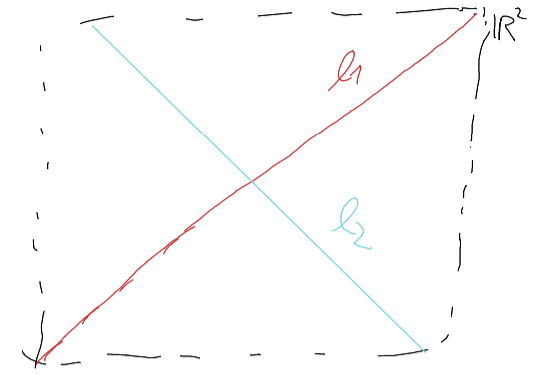
\includegraphics[width=.7\textwidth]{sketch_6_01.png}
    \caption{Sketch 6.01}
\end{figure}
\begin{figure}[H]
    \centering
    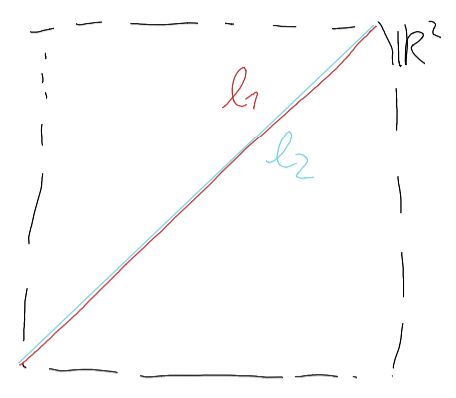
\includegraphics[width=.7\textwidth]{sketch_6_02.png}
    \caption{Sketch 6.02}
\end{figure}
\begin{figure}[H]
    \centering
    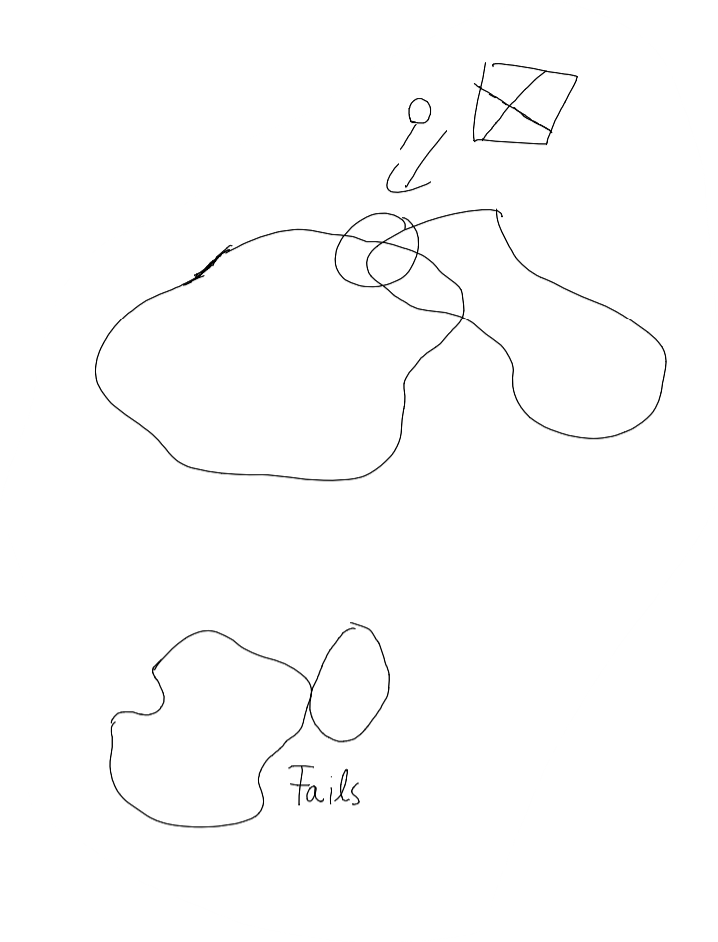
\includegraphics[width=.7\textwidth]{sketch_6_03.png}
    \caption{Sketch 6.03}
\end{figure}
\dhighlight{Observations:}
\begin{enumerate}
    \item transversality is stable (slight changes to the lines don't change transversality) \marginnote{Similarly to being full rank}
    \item transversality is generic(for pretty much any lines \(l_1,l_2\) they are transverse)
\end{enumerate}

One goal: Develop non-linear theory  of transversality. I.e. replace \(l_1,l_2\subset\R^2\) by manifolds.

Both of the above observations will still be true.  % sketches ...

\markeol{10}

\beginlecture{11}{15.11.2024}

\dhighlight{Announcement} On Tuesday, November 26, there will be a course evaluation. 

\begin{itemize}
    \item Please show up that day!
    \item Bring a phone / computer
\end{itemize}

\subsection{Transversality for submanifolds}

Let \(M\) be a smooth manifold. 
\begin{definition*}
    We say that a pair of submanifolds \(K,L\subset M\) are \dhighlight{transverse} at \(p\in K\cap L\) if 
    \marginnote{Here the sum is a gain the span of both of them}\[T_p K + T_p L = T_p M.\]
    We say that \(K,L\) are \dhighlight{transverse} and write \(K\pitchfork L\).
\end{definition*}

\begin{remark}
    In the literature, we  also see ``transversal'', ``transversally intersecting''. 
\end{remark}

\begin{example}
    \begin{figure}[H]
        \centering
        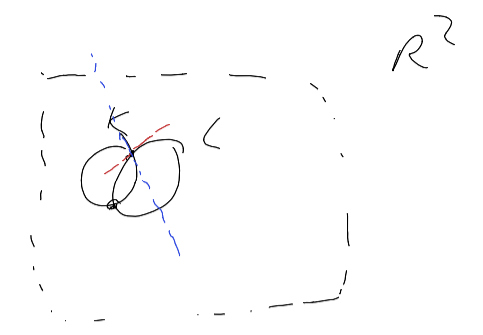
\includegraphics[width=.7\textwidth]{sketch_6_05.png}
        \caption{Sketch 6.05}
    \end{figure}
    \(K,L\) are transverse.
    \begin{figure}[H]
        \centering
        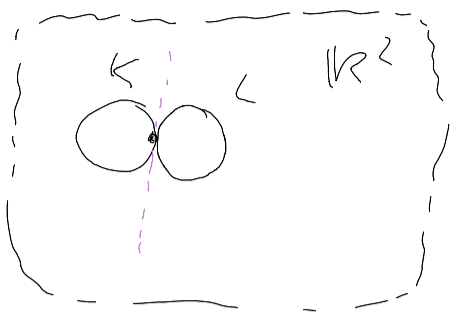
\includegraphics[width=.7\textwidth]{sketch_6_06.png}
        \caption{Sketch 6.06}
    \end{figure}
    \(T_p K=T_P L\), transversality fails.
\end{example}

\begin{lemma}\label{lem:6.1}\marginnote{Key lemma for transversality}
    Let \(K^k,L^l\) be submanifolds of \(M\). If \(K,L\) are transversal, then 
    \(K\cap L \subset M\) is a submanifold.
\end{lemma}

\begin{remark}
    In general, if \(S,T\) are submanifolds of \(N\), then \(S\cap T\) need not be a topological submanifold.
    For example: \(f:\R^2\to R\)
    \[f(x,y)=x^2-y^2.\]
    Let \(g:\R^2\to \R\) 
    \[g(x,y)=0.\]
    Let \(S=\{(x,y,z)\mid z=f(x,y)\}\subset \R^{2+1}\) and \(T=\{(x,y,z)\mid z=g(x,y)\}\subset \R^{2+1}\).
    But \[S\cap T=\{(x,y,z)\mid z=0,x^2-y^2=0\}\]
    \begin{figure}[H]
        \centering
        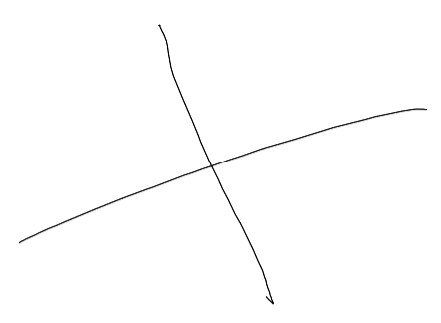
\includegraphics[width=.7\textwidth]{sketch_6_07.png}
        \caption{Sketch 6.07}
    \end{figure} 
    Look at the derivative at 0 .... % TODO
\end{remark}

\begin{proof}
    This is a local question, e.g. by theorem \ref{thm:5.3}. So we may as well assume that \(M=U\subset \R^n\).
    We can also assume that \(0\in U\).
    
    It is enough to check that \(K\cap L\) smooth submanifold in a neighborhood of \(p=0\). By rank theorem (\ref{thm:4.3}), we may assume 
    (after possibly further shrinking \(U\ni 0\)) that \(K=f^{-1}(0),f:U\to\R^{n-k}\),
    \(L=g^{-1}(0), g:U\to\R^{n-l}\) where \(f,g\) have full rank.

    \begin{figure}[H]
        \centering
        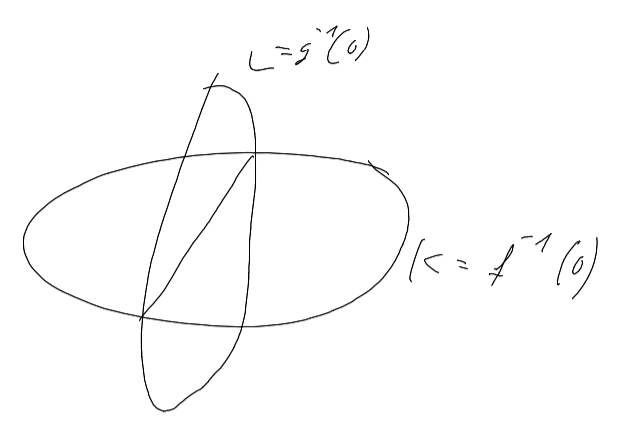
\includegraphics[width=.7\textwidth]{sketch_6_08.png}
        \caption{Sketch 6.08}
    \end{figure}
    Now we consider \(H=(f,g):U\to \R^{n-k}\oplus \R^{n-l}\). It is enough to prove that \(dH_0\) is 
    surjective (by the rank theorem). Note that \(H^{-1}(0)=f^{-1}(0)\cap g^{-1}(0)=K\cap L\).

    To see surjectivity of \(dH_0\), we consider the exact sequences: 
    \begin{figure}[H]\label{fig:6.09}
        \centering
        \begin{tikzcd}
            \arrow[ddd,swap,sloped,"="]\arrow[ddd,sloped,"transversality"]T_0L + T_0K \arrow[r] & T_0L/{(T_0L\cap T_0 K)} \oplus T_0K/{(T_0L\cap T_0 K)}  \arrow[ddd,"(df_0{,}dg_0)"]\\
            &\\
            &\\
            \R^m \equiv T_0U \arrow[r,"dH_0=(df_0{,}dg_0)"] & R^{n-k}\oplus \R^{m-l}
        \end{tikzcd}
        \caption{Sketch 6.09}
    \end{figure}
    The horizontal map \(T_0 L + T_0 K\to T_L/(T_0L\cap T_0K)\oplus T_K/(T_0L\cap T_0K)\) sends \(v+w\)
    to \((v,w)\). This is well defined, because if \(v+w=v'+w'\implies v-v'=w-w'\in T_0L\cap T_0K\). (Equivalently, this map is 
    just quotient by \(T_0L\cap T_0K\))

    Clearly the R.H vertical arrow is injective: the kernel of \(df_0=T_0K\), so \((df_0)\restrict{T_0L/(T_0L\cap T_0K)}\) and similarly for \(dg_0\).
    To prove the R.H. vertical arrow is an isomorphism, do a dimension count:\marginnote{Exact sequence} 
    \begin{center}
        \begin{tikzcd}
            0 \arrow[r]&  T_0K\cap T_0L \arrow[rr,"v \mapsto (v{,}v)"] && T_0K + T_0L\arrow[rr,"(u{,}w)\mapsto u-w"]&& T_0U\equiv \R^n\arrow[r]& 0
        \end{tikzcd}
    \end{center}
    \(\implies \dim(T_0K\cap T_0L)+n=k+l\implies \dim(T_0L/_{(T_0K\cap T_0L)})=l-(k+l-n)=n-k\) and \(\dim(T_0K/_{(T_0K\cap T_0L)})=k-(k+l-n)=n-l\).
    We conclude that the R.H. vertical arrow is an isomorphism. 
\end{proof}

\begin{remark}
    We have 
    \begin{figure}[H]\label{fig:6.10}
        \centering
        \begin{tikzcd}
            \arrow[d,sloped,"\sim"] T_0L\cap T_0 K\arrow[r,hook] &\arrow[d,sloped,"\sim"] T_0L+ T_0K\\
            \ker(dH_0)\arrow[r,hook] & T_0U\equiv \R^3
        \end{tikzcd}
        \caption{Sketch 6.10}
    \end{figure}
    where the left vertical arrow is an isomorphism, due to the five lemma or diagram chasing.

    Hence \(\ker (dH_0)=T_0L\cap T_0K=T_0(L\cap K)\).
\end{remark}

\subsection{Transversality of maps}

\begin{definition*} % TODO: FIX
    Let \begin{figure}[H]\label{fig:6.11}
        \centering
        \begin{tikzcd}
            & Y \arrow[d,"g"]\\
            X\arrow[r,"f"] & Z
        \end{tikzcd}
        \caption{Sketch 6.11}
    \end{figure}
    be a diagram in Top (the category of topological spaces). We let \(X\times_Z Y \coloneqq \{(x,y)\mid f(x)=g(y)\}\subset X\times Y\),
    endowed with the subspace topology. We call \(X\times_Z Y\) the \dhighlight{fiber product (of the diagram)}.
\end{definition*}

\begin{remark}[for enthusiasts only]
It can be shown that given any topological space \(W\in \text{Top}\) and maps 
\begin{center}
    \begin{tikzcd}
        W \arrow[d]\arrow[r] & Y\arrow[d]\\ 
        X \arrow[r,]& Z
    \end{tikzcd}
\end{center}
\begin{figure}[H]\label{fig:6.12}
    \centering
    
    \begin{tikzcd}
        W\arrow[rdd,bend right]\arrow[rrd,bend left]\arrow[dr,dashed,sloped,"\exists!"]&&\\
        &X\times_ZY\arrow[d]\arrow[r] & Y\arrow[d]\\ 
        &X \arrow[r]& Z
    \end{tikzcd}
    \caption{Sketch 6.12}
\end{figure}

there exists a unique map \(W\to X\substack{\times\\ z} Y\) commutes.(Universal property)
\end{remark}

Lots of categories admit fiber products! This is a good property for categories to have. 

\dhighlight{Bad news:} The (not-full) subcategory \(\maninf\subset\text{Top}\) does not admit 
fiber products (nor does \(\man0\subset\text{Top}\)). 
\begin{example}[Non-example]
    \(Z=\R^{2+1},X=\text{graph}(x^2-y^2),Y=\text{graph(0)}\).
\end{example} 

\begin{definition*}
    Let \begin{figure}[H]\label{fig:6.13}
        \centering
        \begin{tikzcd}
            & Y \arrow[d,hook',"g"]\\
            X\arrow[r,hook,"f"] & Z
        \end{tikzcd}
        \caption{Sketch 6.13}
    \end{figure}
    be a diagram in \(\maninf\). We say that \(f,g\) are \dhighlight{transverse} at \(z=f(x)=g(y)\) if 
    \[\text{im }df_x+\text{im }dg_y=T_zZ.\]
    We say that \(f,g\) are \dhighlight{transverse} and say \(f\pitchfork g\) if this holds 
    for all such \(z\).
\end{definition*}

\begin{remark}
    Transversality for maps generalizes transversality for submanifolds. Take the diagram 
    \begin{figure}[H]\label{fig:6.14}
        \centering
        \begin{tikzcd}
            & Y \arrow[d,hook']\\
            X\arrow[r,hook] & Z
        \end{tikzcd}
        \caption{Sketch 6.14}
    \end{figure}
\end{remark}

\begin{proposition}\label{prop:6.2}
    If \(f\pitchfork g\), then \(X\times_Z Y \stackrel{i}{\to} X\times Y\) is a smooth embedding.
\end{proposition}
\marginnote{The diagonal arrows are the obvious projections}
\begin{figure}[H]\label{fig:6.15}
    \centering
    \begin{tikzcd}
        &Y&\\
        X \times_ZY\arrow[rr,hook]\arrow[ur] &&X\times Y\arrow[lu] \\
        &\arrow[lu]X\arrow[ru]&
    \end{tikzcd}
    \caption{Sketch 6.15}
\end{figure}

\begin{proof}
    Some observations:
    \begin{itemize}
        \item exercise sheet 07: \(X\times_ZX\times Y\) is proper.
        \item similarly to the proof of theorem \ref{thm:5.6:whithney}, it is enough to prove that 
              \(i\) is an injective immersion. By definition \(i\) is injective. Therefore we need to check that \(i\) is smooth and the differential is injective.
    \end{itemize}

    Consider 
    \begin{figure}[H]\label{fig:6.16}
        \centering
        \begin{tikzcd}
            \Delta\coloneqq (X,Y,Z,Z)\arrow[d,bend right] &\\
            X\times Y\times Z\times Z\arrow[r,"\pi"] & X\times Y \\
            W=\text{graph}(f,g)\arrow[u,bend left]&
         \end{tikzcd} 
        \caption{Sketch 6.16}
    \end{figure}        
    where \[\text{graph}(f,g)=\coloneqq \{(x,y,x_2,z_1,z_2)\mid z_1=f(x),z_2=g(y)\}.\]
    Then \[W\cap \Delta=\{(x,y,z_1,z_2)\mid z_1=z_2=f(x)=g(y)\}=X\times_ZY.\]
    We have:
    \begin{figure}[H]\label{fig:6.17}
        \centering
        \begin{tikzcd}
            W\cap \Delta \arrow[rr, hook,"j"] \arrow[d,sloped,"\sim"]\arrow[d,swap,"\alpha"]\arrow[rd,hook,"i"] & & X\times X\times Z\times Z \arrow[ld,"\pi"]\\
            X\times_ZY\arrow[r,hook] & X\times Y
        \end{tikzcd}  
        \caption{Sketch 6.17}
    \end{figure} 
    \(\alpha\) is clearly bijective and continuous. It is elementary that \(\alpha\) is a closed map.
    That means we have to check the limit points. \(W\cap \Delta\) is closed, i.e. contains the same limit points\dots   
    Therefore \(\alpha\) is a homeomorphism.

    By lemma \ref{lem:6.1}, if we can show that \(W\pitchfork \Delta\), then \(W\cap \Delta\stackrel{j}{\hookrightarrow}X\times Y\times Z\times Z\) is smooth embedding. 
    Hence \(i\coloneqq \pi\circ j\) smooth. Let us now check that \(W\pitchfork \Delta\) at some arbitrary point \(p=(x,y,z,z)\in W\cap \Delta\subset X\times Y\times Z\times Z\).
    Note that \(z=f(x)=g(y)\). We have \[T_pW=\{(v,w,df_x(v),dg_y(w))\}\]
    and 
    \[T_p\Delta=\{v',w',u,u\},\]
    where \(v,v'\in T_xX,w,w'\in T_yY,u\in T_zZ.\)
    We need to check: \(T_p W+T_p\Delta=T_p(X\times Y\times Z\times Z)\). 
    We must show that for an arbitrary \((a,b,c,d)\in T_p(X\times Y\times Z\times Z)=T_xX\oplus T_yY\oplus T_zZ \oplus T_zZ.\)

    \markeol{11}\beginlecture{12}{19.11.2024}

    We must solve: 
    \begin{align*}
        a&=v+v'\\
        b&=w+w'\\
        c&=u+df_x(v)\\
        d&=u+dg_y(w)
    \end{align*}
    for some \(\underbrace{(v,w,df_x(v),dg_y(w))}_{\in T_pW}, (v',w',u,u)\in T_p\Delta\).
    The above is equivalent to \marginnote{we solve this, since we want to show \(f\pitchfork g\iff \forall z\in X\times_ZY:\text{im} df+\text{im}dg=T_zZ\)}
    \begin{align*}
        c-d  & = df_x(v)-dg_y(w)\in T_zZ & \text{By assumption there exists \(v,w\) s.t. equation holds}\\
        c+d &=2u+df_x(v)+dg_y(w) & \text{can solve by picking suitable } u \\
        a-v&=v'&\\
        b-w&=w' & \text{choose } v',w'\text{ s.t. this holds}\\ 
    \end{align*}   % TOFIX (photo)
    Follows from Lemma \ref{lem:6.1} that
    \begin{center}
        \begin{tikzcd}
            \Delta\cap W\arrow[r,hook]\arrow[rr,bend right,"i"] & X\times Y\times Z\times Z \arrow[r,"\pi"] & X\times Y
        \end{tikzcd}
    \end{center}
    is a smooth submanifold. Finally, \(d_i\) is injective. This is clear, because \begin{tikzcd}
    T_pW\arrow[r] & T_{(x,y)} X\times Y
    \end{tikzcd} is injective. Indeed, if \((v,w,df_x(v),dg_y(w))\mapsto 0\), then \((v,w)=(0,0)\), but then 
    \((v,w,df_x(v),dg_y(w))=(0,0,0,0)\).
\end{proof}

\section{Sard's theorem}

\subsection{Measure theory on manifolds}

\begin{definition*}
    A subset $S\subset \R^n$ has \dhighlight{measure zero} if, for any \(\epsilon>0\), there exists a family 
    \(\{C_i\}_{i=1}^\infty\) of rectangles:
    \[\R^n\supset C_i = (a_1^i-\epsilon_1^i,a_1^i+\epsilon_1^i)\times\dots\times (a_n^i-\epsilon_n^i,a_n^i+\epsilon_n^i),\]
    where \((a_1^i,\dots,a_n^i)\in\R^n\) and \((\epsilon_1^i,\dots,\epsilon_n^i)\in\R_{>0}^n\), s.t. 
    \[S\subset \bigcup_{i=1}^\infty C_i\land \sum_{i=1}^\infty \text{vol}(C_i)<\epsilon.\] 
\end{definition*}

\begin{remark}
    We would get an equivalent definition, if we replaced rectangles with balls, cubes, paralellograms,\dots.
\end{remark}

\begin{example}
    Suppose \(S\subset\R^1\) and \(|S|<\infty\), clearly S now has measure zero: \(a_i\in S\implies (a_i-\epsilon,a_i+\epsilon)\) has finite volume \(2n\epsilon\).
    \begin{itemize}
        \item \(S\subset\R\), \(S\) countable. Then \(S\) has measure zero: Take \((a_i-\frac{\epsilon}{2^i},a_i+\frac{\epsilon}{2^i})\)
    \end{itemize}
\end{example}

\begin{lemma}\label{lem:6.3}
    \begin{enumerate}
        \item[(i)] If \(A\subset B\subset\R^n\) and \(B\) has measure zero, then \(A\) has measure zero. 
        \item[(ii)] if \(A\subset\R^n\) is a countable union of measure zero subsets, then \(A\) also has zero measure.   
    \end{enumerate}
\end{lemma}

\begin{proof}
    Emitted.
\end{proof}

\begin{lemma}\label{lem:6.4}
    Let \(A\subset \R^n\) be compact. Suppose that for all \(c\in\R:A\cap\{c\}\times \R^{n-1}\)
    has \((n-1)\)-dimensional measure zero. Then \(A\) has \(n\)-dimensional measure zero. 
\end{lemma}

\begin{figure}[H]\label{fig:6.18}\marginnote{This is misleading \dots}
    \centering
    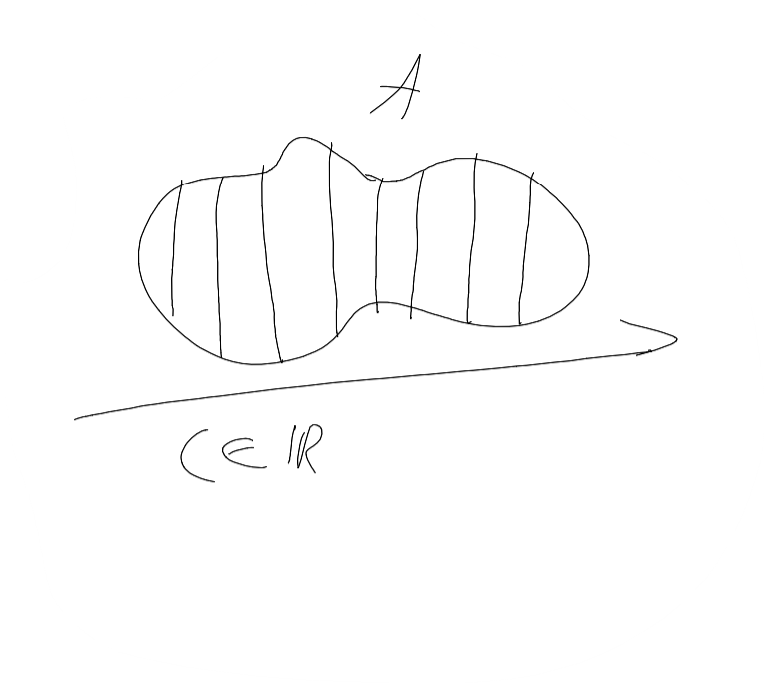
\includegraphics[width=.7\textwidth]{sketch_6_18.png}
    \caption{Sketch 6.18}
\end{figure}
\begin{figure}[H]\label{fig:6.19}
    \centering
    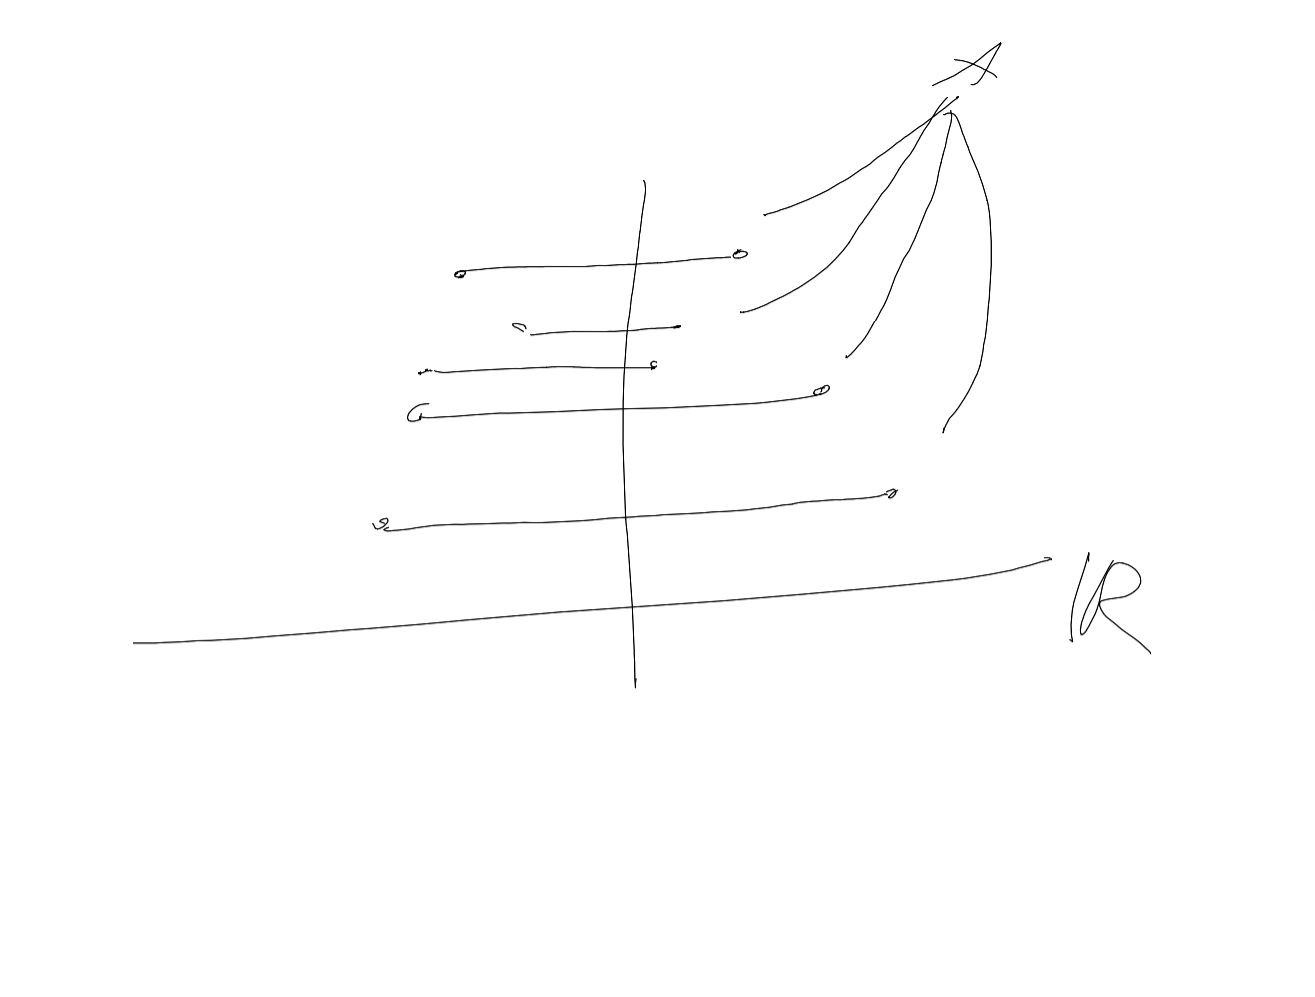
\includegraphics[width=.7\textwidth]{sketch_6_19.png}
    \caption{Sketch 6.19}
\end{figure}

\begin{proof}
    Choose \(a<b,a,b\in \R\) so that \(A\subset (a,b)\times \R^{n-1}.\) Let \(A_c\coloneqq\{x\in\R^{n-1}:(c,x)\in A\}.\)
    Fix \(\epsilon>0.\) By assumption, we can cover \(A_c\) by a union of rectangles \(U_c\coloneqq \bigcup_{i=1}^\infty C_c^i\)
    such that \(\sum_{i=1}^\infty\text{vol} (C_i)<\epsilon\).

    By compactness there exists an open interval \(J_c\) such that \(A\cap J_c\times \R^{k-1}\subset J_c\times U_c.\)
    \begin{figure}[H]\label{fig:6.20}
        \centering
        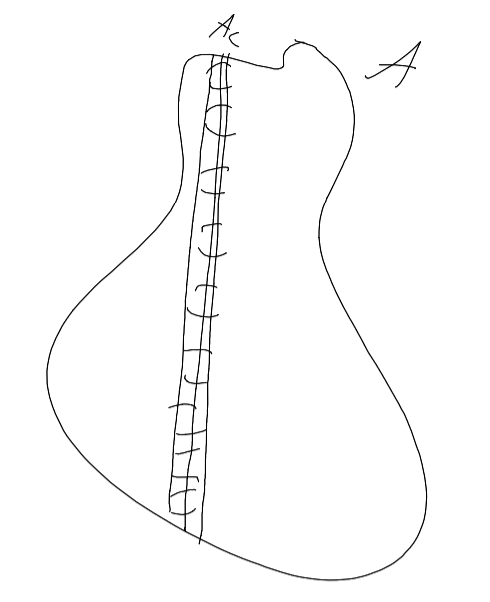
\includegraphics[width=.7\textwidth]{sketch_6_20.png}
        \caption{Sketch 6.20}
    \end{figure}
    Otherwise, there exists a sequence \((c_i,x_i),c_i\to c\land x_i\notin U_c\land (c_i,x_i)\in A\). By compactness one can extract a 
    convergent subsequence \(\to (c,x)\in A\)\marginnote{Since \(A\) compact}, \(x\in U_c^C\). This is impossible, since 
    \(A\subset U_c\). 

    By compactness of \([a,b]\), there is a finite sequence \(a=c_1<c_2<\dots<c_l=b\) such that 
    \[\bigcup_{i=1}^l J_{c_i}\text{ covers } [a,b].\]
    We can freely assume up to deleting certain \(J_{c_i}\) that \(\sum \text{vol}(J_{c_i})<2|b-a|\). 
    \marginnote{He writes \(|J_{c_i}|\) \dots}
    Finally: \(A\subset \bigcup_{i=1}^l J_{c_i}\times U_{c_i}\). But 
    \[\text{vol}(J_{c_i}\times U_{c_i})\leq \sum |J_{c_i}|\times |U_{c_i}|\leq \epsilon\sum |J_{c_i}|=2\epsilon|b-a|\]
\end{proof}

\begin{corollary}\label{cor:6.5}
    Let \(f:\underbrace{A}_{\subset \R^n}\to\R^{1}\), where \(A\) is a countable union of compact subsets (e.g. A could be open or closed) and \(f\) continuous.
    Then the graph of \(f\): \[\text{graph}(f)=\{(x,y)\mid y=f(x)\}\]
    has measure zero as a subset of \(\R^{n+1}\). \marginnote{\(\R^n\times\{c\}\subset\R^{n+1}\) is a measure zero set}
\end{corollary}

\begin{proof}
    Assume \(A\) compact. Argue by induction. If \(n=0\), trivial. Assume that the result holds for \(\leq n+1\).
    Observe that \(\forall c\in\R\), \(\text{graph}(f)\cap\{c\}\times \R^{(n-1)+1}=\text{graph}\left(f\restrict{\{c\}\times \R^{n-1}}\right)\), which by induction has measure zero. 
    Hence follows from Lemma \ref{lem:6.4}. For general \(A\), write \(A=\bigcup_{i=1}^\infty K_i\). Then \marginnote{Holds by Lemma \ref{lem:6.3}}
    \[\text{graph}(f)=\bigcup_{i=1}^\infty\underbrace{\text{graph}\left(f\restrict{\{K_i\}}\right)}_{\text{measure zero}}\]
\end{proof}

\begin{lemma}\label{lem:6.6}
    Let \(A\subset\R^n\), let \(F:A\to\R^n\) be smooth. If \(A\) has measure zero, so does \(F(A)\).
\end{lemma}

\begin{remark}
    Smoothness is important. The lemma would be false if we only assume \(F\) to be continuous. Example: 
    \(F\) the cantor function. Smoothness is way to strong. Absolutely continuous functions are the correct class.
\end{remark}

\begin{proof}[Proof of lemma \ref{lem:6.6}]
    By definition, for any \(p\in A\), \(F\) extends to a smooth map on a neighborhood of \(p\). Up 
    to shrinking this neighborhood \(U_p\) that \(F\) extends to \(\overline{U_p}\). We can also assume that 
    \(U_p\) is a ball. Note that \(A\subset \bigcup_{p\in A} U_p\). By lemma \ref{lem:1.5}, we can extract 
    a countable subcover. Hence it is enough to prove that \(F(A)\cap U_p\) has measure zero for 
    all \(p\in A\). 

    By Taylor's theorem\marginnote{Here we use smoothness}, \(F\) is uniformly continuous on \(\overline{U_p}\),
    and we have 
    \begin{equation}\label{eq:proof_lem6.6}
        |F(x)-F(y)|< Q|x-y|  
    \end{equation}
    for all \(x,y\in\overline{U_p}\). Fix \(\delta>0\). Since \(A\cap \overline{U_p}\) has measure zero, 
    can cover \(A\cup \overline{U_p}\) by a countable union of balls \(C_i\), such that  
    \(\sum_{i}\text{vol}(C_i)<\delta.\) By (\ref{eq:proof_lem6.6}), \[\text{diam}(F(\overline{U_p}\cap C_i))<Q'\text{diam}(C_i)\],
    where \(Q'\leq 100Q\). \(\implies F(A\cap \overline{U_p})\) is contained in a countable union of balls \(D_i\)
    of diameter \(\leq Q'\text{diam}(C_i)\). Hence 
    \[\sum_{i=1}^\infty\text{vol}(D_i)<Q'\sum\text{vol}(C_i)<100^n Q'\delta.\qedhere\]

\end{proof}

\begin{definition*}
    Let \(M\) be a manifold. A subset \(S\subset M\) has measure zero, if, for all charts \((U,\phi)\),
    \(\varphi(S\cap U)\) has measure zero in \(\R^n\).
    \begin{figure}[H]\label{fig:6.21}
        \centering
        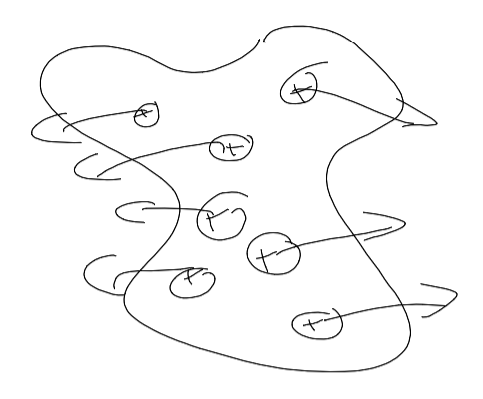
\includegraphics[width=.7\textwidth]{sketch_6_21.png}
        \caption{Sketch 6.21}
    \end{figure}
\end{definition*}

\begin{lemma}\label{lem:6.7}
    If \(\cA\subset\cA'\) is an inclusion of atlases. Then \(S\) has measure zero w.r.t. \(\cA\iff\) S has measure zero w.r.t. \(\cA'\).
\end{lemma}

\begin{proof}%maybe add sketch 6.22
    Assume that \(S\) has measure zero w.r.t. \(\cA\), i.e. \(\phi_\alpha(S\cap U_\alpha)\) has measure zero for all charts 
    \((U_\alpha,\phi_\alpha)\). Assume \((V,\psi)\) is a chart for \(\cA'\). Then 
    \begin{align*}
        \psi(S\cap V)&=\psi\left(\bigcup_{\alpha\in\cA} (U_\alpha\cap S)\cap V\right)\\
                     &=\psi\left(\bigcup_{\alpha\in\cA} (U_\alpha\cap S\cap V)\right)\\
                     &=\psi\left(\bigcup_{\alpha\in\cA} \phi_\alpha^{-1}\circ \phi_\alpha (U_\alpha\cap S\cap V)\right)\\
                     &=\bigcup_{\alpha\in\cA} \underbrace{\psi\circ\phi_\alpha^{-1}\left( \phi_\alpha (U_\alpha\cap S\cap V)\right)}_{\text{measure by smoothness}}
    \end{align*}
    because the \(U_\alpha\) form a cover of \(M\), up to replacing \(\cA\) by a countable cover.
\end{proof}
\markeol{12}

\beginlecture{13}{22.11.2024}

\begin{lemma}\label{6.8}\marginnote{Compare lemma \ref{lem:6.6}}
    Let \(M,N\) be smooth manifolds and \(f:M\to N\) a smooth map. If \(A\subset M\)
    has measure zero, then \(F(A)\subset N\) also has measure zero.
\end{lemma}

\begin{proof}
    Fix \(\{(U_\alpha,\varphi_\alpha)\}\) a countable atlas for \(M\). We need to show 
    that given any chart \((V,\psi)\) on \(N\), \(\psi(V\cap F(A))\) has measure zero.
    We may as well assume that \(F(A)\subset V\) (otherwise replace \(A\) with \(F^{-1}(A)\cap V\)).
    Observe that \(\psi(F(A))\) is the countable union of these sets \(\psi(F(\phi_i^{-1}(\phi_i(A\cap U_i))))\):
    \[\psi(F(A))=\bigcup_{i}\psi(F(\phi_i^{-1}(\phi_i(A\cap U_i)))).\]
    But \(\phi_i(A\cap U)\) has measure zero and \(\psi\circ F\circ \phi_i^{-1}\) is a smooth function, which is applied 
    to a subset of measure zero of \(\R^n\). Therefore the set has measure zero by lemma \ref{lem:6.6} along with 
    the fact that countable unions of measure zeros subsets have measure zero (lemma \ref{lem:6.3}).
\end{proof}
\subsection{Sard's theorem}

\begin{definition*}\marginnote{This coincides with the analyis 1 definition}
    Let \(F:M\to N\) be smooth. Given a point \(x\in M\), we say that \(x\) is a \dhighlight{critical point} 
    of \(F\), if the differential  \(dF_x:T_xM\to T_{F(x)}N\) fails to be surjective. Otherwise 
    we say that \(x\) is a \dhighlight{regular point}.
    
    A point \(y\in N\) is a \dhighlight{critical value} if \(F^{-1}(y)\) contains a 
    critical point. Otherwise we say \(y\) is a \dhighlight{regular value}. 
\end{definition*}

\begin{remark}
    If \(F^{-1}(y)=\emptyset\implies y\) is a regular value, but not the image of a regular point!
\end{remark}

\begin{theorem}[Sard]\label{thm:6.9:Sard}\marginnote{Very important theorem}
    Let \(M,N\) be smooth manifolds. Let \(F:M\to N\) be a smooth map. Then 
    the set of critical values of \(F\subset N\) has measure zero. 
\end{theorem}

\begin{example}
    \(M\to\R, M\ni x\mapsto 0\in\R\). Here the set of \dhighlight{critical points} has full measure (since it is \(M\)),
    But the set of \dhighlight{critical values} is \(\{0\}\subset\R\).
\end{example}

\begin{example}
    \begin{figure}[H]\label{fig:6.22} % 6 critical points!
        \centering
        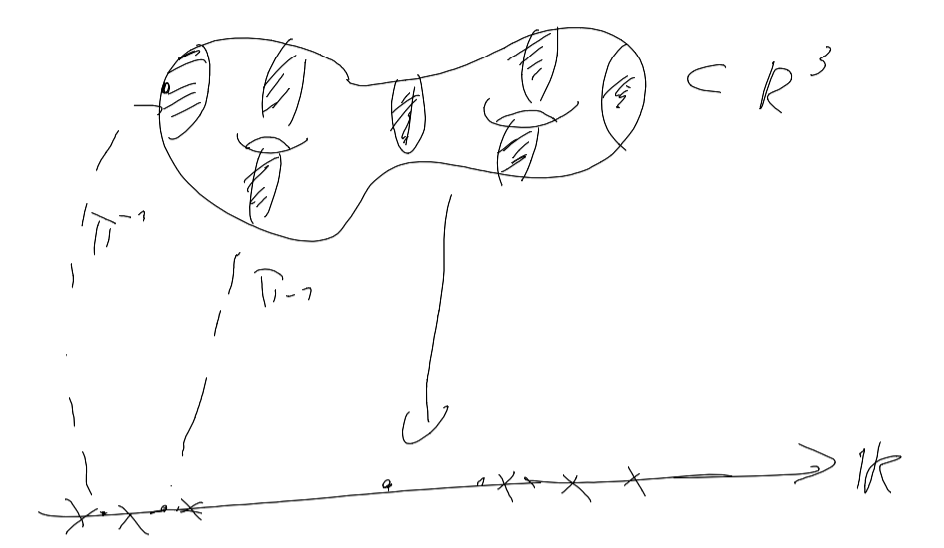
\includegraphics[width=.7\textwidth]{sketch_6_22.png}
        \caption{Sketch 6.22}
    \end{figure}
    Morse theory: study  the topology of manifolds by studying functions on them.
\end{example}

\begin{corollary}\label{cor:6.10}
    Let \(F:M^m\to N^n\) be a smooth map. If \(m<n\), then 
    \(\text{im}(F)\subset N\) has measure zero. 
\end{corollary}

\begin{proof}
    Clear for dimensional reasons.
\end{proof}

\begin{corollary}\label{cor:6.11}
    Let \(M^m\subset \R^N\) be a submanifold. Write \(\R^{N-1}=\{(x_1,\dots,x_{N-1},0)\}\subset\R^N\).
    Given \(v\in\R^{N}-\R^{N-1}\), we set \(\pi_v:\R^N\to\R^{N-1}\) to be the projection with kernel \(\R\cdot v\).
    \begin{figure}[H]\label{fig:6.23}
        \centering
        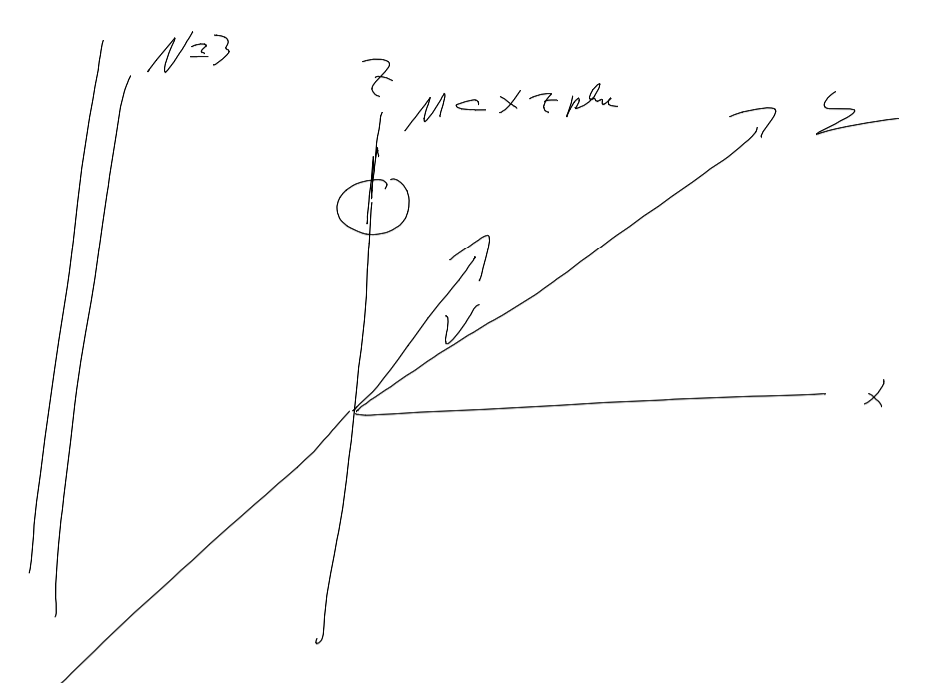
\includegraphics[width=.7\textwidth]{sketch_6_23.png}
        \caption{Sketch 6.23}
    \end{figure}
    Assume that \(N>2m+1\). Then the set of \(v\in\R^{N}\setminus\R^{N-1}\) such that \(\pi_{v\mid_M}:M\to\R^{N-1}\)
    is an injective immersion is non-empty. It is, in fact, dense\footnote{In \(\R\bP^{N-1}, \R^{N}\)}.

\end{corollary}

\begin{example}
    Take \(v=(0,0,1)\). Then \(\pi_{(0,0,1)}(M=S^1)=[-1,1]\), and not injective.
\end{example}

\begin{example}
    \(v=(1,1,1),\pi_v(M=S^1)=S^1\), up to scaling of the axis. %TODO: Detail
\end{example}

\begin{proof}
    Firstly, \(\pi_{v\mid_M}\) is injective \(iff\) for all 
    \(p\in M\), \((p+tv)_{t\in\R}\cap M = \{p\}\). 
    
    Secondly,
    \(\pi_{v\mid_M}\) is an immersion \(\iff\) for all \(p\in M\), \(T_pM\cap \ker d\pi_v=0\)\footnote{i.e. the zero vector space}
    \(\iff \overbrace{T_pM}^{\subset\R^N}\) does not contain \(v\).

    Let \(\Delta\subset M\times M\) be the diagonal (i.e. \(\Delta=\{(x,x)\mid x\in M\}\subset M\times M\)). Let 
    \(0_M\subset TM\) be the \dhighlight{zero section}: 
    \[0_M\coloneqq \{(p,0)\in TM\}\subset TM\]
    where \[TM=\bigcup_{p\in M} T_p M.\]
    \begin{figure}[H]\label{fig:6.24}
        \centering
        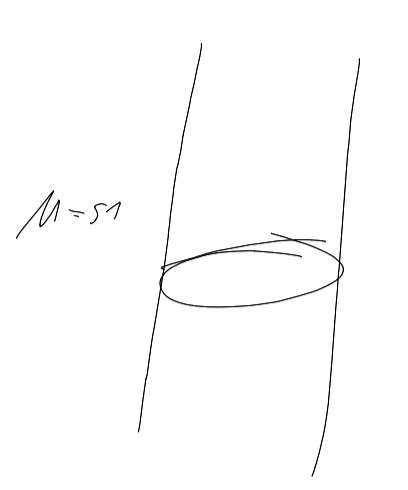
\includegraphics[width=.7\textwidth]{sketch_6_24.png}
        \caption{Sketch 6.24}
    \end{figure}
    Define \begin{align*} % TODO: fix
        \alpha:& M\times M \setminus \Delta \to  \R\bP^{N-1}\\
        &(p,q)\mapsto [p-q]\\
        \beta:& TM\setminus O_M\to \R\bP^{N-1}\\
        &(p,w)\mapsto  [w]
    \end{align*}
    It is easy to check that \(\alpha,\beta\) are smooth. Check \(\alpha\)
    \begin{align*}
        (p,q)\mapsto \underbrace{p-q}_{\in\R^{N}-\{0\}}\mapsto \underbrace{[p-q]}_{\in\R^N\setminus \{0\}/\R^\times}\equiv \R\bP^{N-1}.
    \end{align*}
    \marginnote{To see that quotient maps are smooth is a good exercise for the exam}
    Note that \(N-1>2m\), and dimension of \(M\times M\setminus\Delta\) and \(TM-O_M\) is \(2m\).
    It follows by corollary \ref{cor:6.10} that \(\text{im}(\alpha)\cup\text{im}(\beta)\subset \R \bP^{N-1}\) has measure zero.
    Finally the conclusion follows from sheet 08.
\end{proof}

\begin{corollary}[Strong Whitney embedding]\label{cor:6.12:strong_whitney}
    Suppose that \(M^m\) (compact) manifold. Then \(M\) admits an embedding into \(\R^{2m+1}\).
\end{corollary}

\begin{remark}
    Compactness is not a necessary assumption. But our prof. assumes compactness. If we use this, we don't have to use compactness.
\end{remark}

\begin{proof}
    By theorem \ref{thm:5.6:whithney}, \(M\) admits an embedding into \(\R^N\), \(N\gg1\). If \(N>2m+1\),
    then by corollary \ref{cor:6.11} there exists \(v\in\R^N\setminus\R^{N-1}\), such that \(\pi_{v\mid_M}:M\to\R^{N-1}\)
    is an injective immersion. By repeatedly applying corollary \ref{cor:6.11}, we get an 
    injective immersion from \(M\stackrel{i}{\hookrightarrow} \R^{2m+1}\). As in the proof of theorem \ref{thm:5.6:whithney},
    \(i\) must be an embedding, because \(M\) is compact.
\end{proof}

\begin{corollary}\label{cor:6.13} Let \(I,X,Y,Z\) be manifolds. Let \(f:X\times I\to Z,g:Y\to Z\)
    be smooth maps. Suppose that \(f\pitchfork g\). Then for almost all \(s\in I\)\marginnote{i.e. away from a set of measure zero}
    \[f_s(\cdot)=f(\cdot,s)\pitchfork g.\] 
\end{corollary}

\begin{remark}
    Let \(f_0:X\to \R^n,g:Y\to\R^n\) be any maps. Consider \[f:X\times \R^n\to\R,(x,s)\mapsto f_0(x)+s\].
    Then \(f\) is clearly a submersion. Hence \(f\pitchfork\psi\implies f_s\pitchfork g\) for almost all \(s\).
\end{remark}

\begin{proof}
    By assumption and proposition \ref{prop:6.2}: 
    \begin{center}
        \begin{tikzcd}
            W=(X\times I)\times_ZY\arrow[dr,"\pi"] \arrow[rr,hook,"\text{smooth embedding}"] && \arrow[dl](X\times I)\times Y\\
            & I &
        \end{tikzcd}      
    \end{center}
    We will show that if \(s\in I\) is a regular value of \(\pi\), then \(f_S\pitchfork g\). This implies the corollary
    by Sard's theorem \ref{thm:6.9:Sard}.
    
    So suppose that \(s\in I \) is a regular value. Then either 
    \begin{enumerate}
        \item[(i)] \(s\notin\text{im}(\pi)\). In this cae \(\text{im}(f_s)\cap g=\emptyset\)
        \item[(ii)] \(s\in\text{im}(\pi)\). In this case \(d_\pi\)  is surjective on \(\pi^{-1}\). 
    \end{enumerate}
    Let's assume case (ii). Suppose that \(z=f_s(x)=g(y)\). Since  \(f\pitchfork g\), we have 
    \[\text{im}df_x+\text{im}dg_y=T_zZ.\]
    FOr any \(a\in T_zZ\), there exists a pair \(b=(w,e)\subset T_{x,s}(X\times I)=T_xX\oplus T_sI\),
    such that \(df_{(x,s)}(w,e)-a\in \text{im}dg_y.\) 

    Since \(d\pi\) is surjective, there exist an element \((w',e,c')\in T_{(x,s,y)}W=T_{(x,s,y)}(X\times I)\times_ZY\).
    But now \[(df_s)_x(w-w')-a=df_{(x,s)}((w,e)-(w',e))-a=\underbrace{df(\overbrace{b}^{=(w,e)})-a}_{\in \text{im}dg_y}-\underbrace{\overbrace{df(w',e)}^{dg_y(c')}}_{\in \text{im}dg_y}\]
    \begin{center}
        \begin{tikzcd}
            \arrow[d](X\times I) \times_Z Y\arrow[r] & Y\arrow[d]\\
            X\times  I \arrow[r] & Z 
        \end{tikzcd}
    \end{center}
    \(\implies (df_s)_x(w-w')-a\in \text {im}dg_y\).

\end{proof}

\markeol{13}
\beginlecture{14}{26.11.2024}

In this lecture we will try to prove theorem \ref{thm:6.9:Sard} using three intermediate lemmas.

\dhighlight{Notation (auxiliaray):} Consider \(U\subset\R^m\) open, \(F:U\to \R^n\). We let \(C\subset U\)
be the set of critical points of \(F\). More generally, for \(k\geq 1\) we let 
\[C\supset C_k\coloneqq \{x\in C\mid \forall 1\leq i\leq k: \text{All ith partial derivatives of }F\text{ vanish at }x\}.\]
Clearly \(C\supset C_1\subset C_2\subset \dots \). Note also \(C,C_k\) are all closed.\marginnote{Because being zero is a closed condition}
\begin{figure}[H]\label{fig:6.26}
    \centering
    \includegraphics[width=.7\textwidth]{example-image}
    \caption{Sketch 6.26}
\end{figure}

\begin{lemma}\label{lem:6.14}
    Suppose that \(k>\frac{m}{n}-1\). Then \(F(C_k)\) has measure zero.
\end{lemma}

\begin{proof}
    For each \(a\in U\), there exists a closed cube \(a\in E\subset U\). By second countability 
    we can cover \(C_k\) by countability many such cubes. Hence it is enough to prove, for arbitrary 
    such \(E\) that \(F(C_k\cap E)\) has measure zero. Now fix \(a\in C_k\) and cube \(E\ni a\). Also 
    fix \(A>\sup_{y\in E}|\partial_x^{\alpha} F(y)|\) for \(\alpha=(\alpha_1,\dots,\alpha_m)\in \N^m,|\alpha|\leq k+1\).

    Let \(L>0\) be the side length of \(E\). Let \(K\gg 1\) be a natural number.
    We now subdivide \(E\) by \(K^m\) cubes of side length  \(L/K\). Let \(E_1,\dots,E_{K^m}\) be 
    an enumeration of these subcubes.
    \begin{figure}[H]\label{fig:6.27}
        \centering
        \includegraphics[width=.7\textwidth]{example-image}
        \caption{Sketch 6.27}
    \end{figure}
    Since \(a\in E\) there exists some \(i_0\) such that \(a\in E_{i_0}\).
    Since \(a\in C_k\), Taylor's theorem finishes the following inequality:
    \[|F(x)-F(a)|\leq A'|x-a|^{k+1}\] 
    for all \(x\in E_{i_0}\), where \(A'\) depends only on \(A\).

    \(\implies F(E_{i_0})\) is contained in a ball centered at \(F(a)\) of radius \(A'(L/K)^{k+1}\). 
    Now \[F(C_k\cap E)=\bigcup_{i\mid C_k\cap E_i\neq \emptyset} F(C_k\cap E_i).\]\marginnote{Restricting to the cubes which intersect \(C_k\) is a very important step, because otherwise we can't Taylor and have no control over the measure!}
    But each \(F(C_k\cap E_i)\) is contained in a union of balls of volume \(\leq \Lambda\left[A'(L/K)^{k+1}\right]^n\).

    Therefore at most \(K^m\) cubes \(E_i\) which intersect \(C_k\) non-emptily. Hence \(F(C_k\cap E)\)
    is contained in a union of balls of total volume at most 
    \[\Lambda A^{' n} K^m\left[(L/K)^{k+1}\right]^n = \lambda A^{' n} L^{(k+1)n}K^{m-(k+1)n}.\]
    Since \(k> \frac{m}{n}-1\) the exponent of \(K\) is negative and hence increasing \(K\)
    forces the equation above to go to zero.
\end{proof}

\begin{lemma}\label{lem:6.15}
    Assume that Sard's theorem holds for domains of dimension \(<m\). Then \(F(C\setminus C_1)\) has measure zero.
\end{lemma}

\begin{proof}\marginnote{Bird's eye view: Change coordinates, consider modified functions}
    Since \(C_1\) is closed in \(U\), we can assume after replacing \(U\) by \(U\setminus C_1\), that \(C_1=\emptyset\).
    Then we just prove that \(F(C)\), under that assumption, has measure zero. 
    
    Fix \(a\in C\). By assumption that \(C_1=\emptyset\). Up to reordering coordinates in the source and in the target, we can assume 
    that \(\partial_{x_1}F^1(a)\neq 0\).
    Set \(\begin{cases}
        u(x)=F^1(x)&\\
        v^i(x)=x_i  & 2\leq i\leq m
    \end{cases}\). By the inverse function theorem \((u,v)=(u,v^1,\dots,v^m)\)
    forms a coordinate system in some neighborhood \(V_a\) of \(a\). Since the transition matrix is
    \[\begin{bmatrix}
        \partial_{x_1} F^1 & \star & \star &\star \\
        0 & & 1 &
    \end{bmatrix}.\]
    We can assume that \((u,v)\) extend to \(\overline{V_a}\). With respect to 
    these new coordinates \((u,v)\), we have \(F(u,v)=(u,F^2(u,v),\dots,F^n(u,v))\).
    So we have: \(dF(u,v)=\begin{bmatrix}
        1 & 0 &\dots & 0\\
        \star & &  \\
        \vdots && \frac{\partial F^i}{\partial v^j}&\\
        \star & &&
    \end{bmatrix}\) where \(2\leq i\leq n, 2\leq j\leq m\). 
    Therefore \(C\cap \overline{V_a}\) is precisely the set of points such that rank\(\left(\frac{\partial F^i}{\partial v^j}\right)<n-1\). 

    Note that \(F(C\cap \overline{V_a})\) is compact. By lemma \ref{lem:6.4}, if we can show that \(F(C\cap)\cap \{y^1=d\}\)
    has measure zero, then \(F(C\cap \overline{V_a})\) has measure zero. Since \(C\) is covered by countably many such \(V_a\) (by second countability),
    we could conclude that \(F(C)\) has measure zero.

    For \(d\in\R\), \(B_d\coloneqq \{v\mid (d,v)\in \overline{V_\alpha}\}\subset \R^{n-1}\). 
    Set \(F_d(v)\coloneqq (F^2(d,v),\dots,F^n(d,v))\). Since \(F(d,v)=(d,F_d(v))\), we 
    have that the critical values of \(F\restrict{\overline{V_a}}\) that lie in \(\{y^1=d\}\)
    are precisely the points \((d,q)\), where \(q\) are critical values of \(F_d\). 
    By assumption that Sard's theorem \ref{thm:6.9:Sard} holds for dimension \(<m\), since the domain of \(F_d\)
    has dimension \(m-1<m\), \(\{\text{critical values of } F_d\}=\{y_1=d\}\cap F(C\cap \overline{V_a})\) has 
    measure zero. \qedhere

\end{proof}
\begin{lemma}\label{lem:6.16}
    Assume that Sard's theorem holds for domains of dimension \(<m\). For all \(k\geq 1\),
    \(F(C_k\setminus\{F(C_{k+1})\})\) has measure zero.         
\end{lemma}

\begin{proof}
    As in the proof of the previous lemma \ref{lem:6.15}, we can assume \(C_{k+1}=\emptyset\). We will prove 
    under that assumption that \(F(C_k)\) has measure zero.

    Let \(a\in C_k\) be arbitrary. Let \(\sigma:U\to \R\) be a k-th partial derivative of \(F\), with the property that 
    \(\sigma\) has at least one non-vanishing partial at \(a\). I.e. \(\begin{cases}
        \sigma =\partial_x^\alpha F & |\alpha|=k\\
        \partial_{x_i}\sigma(a)\neq 0 &\forall i
    \end{cases}.\) Let \(V_a\) be a neighborhood of \(a\) consisting of regular points of \(\sigma\). Let \(\Sigma\coloneqq \{\sigma^{-1}(0)\}\cap V\). Then \(\Sigma\) is a smooth submanifold in \(V_a\).
    By definition of \(C_k\), we have \((C_k\cap V_a)\subset \sigma^{-1}(0)\cap V_a\).
    
    Moreover \(F(C_k\cap V_a)\) is contained in the set of critical values of \(F\restrict{\Sigma}\) (that's because \(\partial_{x_i}F^j=0\implies dF\restrict{T\Sigma}\equiv 0\)).
    But \(\text{dim}(\Sigma)=\text{dim}(U)-1=m-1\). Hence \(\{\text{ critical values of } F\restrict{\Sigma}\}\) has measure zero, by assumption.
\end{proof}

\begin{proof}[Proof of Sard's theorem \ref{thm:6.9:Sard}]
    We prove it by induction on the dimension of the source. If \(F:M^m\to N^n\), and \(m=0\) the statement is true.

    Let's assume that Sard's theorem has been proven for all manifolds \(F:M^m\to N^n\), where \(m<\tilde{m}\).
    We need to prove it for maps \(\tilde{F}:\tilde{M}\to\tilde{N}\), where \(\dim(\tilde{M})=\tilde{m}\).
    \begin{figure}[H]\label{fig:6.28}
        \centering
        \includegraphics[width=.7\textwidth]{example-image}
        \caption{Sketch 6.28}
    \end{figure}
    By covering source and target by charts, we can assume 
    \begin{itemize}\marginnote{If the intersection is non-empty, we reall need lemma \ref{lem:6.14}} %TODO: Fix spacing of margin
        \item \(\tilde{M}=U\subset\R^m\)
        \item \(\tilde{N}\subset\R^n\).
    \end{itemize}

    Apply lemma \ref{lem:6.14},\ref{lem:6.15},\ref{lem:6.16} to get the claim. \qedhere

\end{proof}

\markeol{14} 